%set document type
\documentclass[titlepage]{report}

%package declarations
\usepackage{blindtext}
\usepackage[a4paper,
left=1.5in,
right=1in,
top=1in,
bottom=1in,
footskip=.25in]{geometry}
\usepackage{graphicx}
\usepackage{indentfirst}
\usepackage[utf8]{inputenc}
\usepackage{lastpage}
\usepackage{setspace}
\usepackage{titling}
\usepackage{tocloft}


%unbold table of contents header & subheaders
\renewcommand{\cfttoctitlefont}{\normalfont\Large}% Remove \bfseries from ToC title
\renewcommand{\cftsecfont}{}% Remove \bfseries from section titles in ToC
\renewcommand{\cftsecpagefont}{}% Remove \bfseries from section titles' page in ToC
%capitalize and center 'list of figures' header, per guidelines
\renewcommand{\listfigurename}{\hfill\normalfont\normalsize LIST OF FIGURES\hfill}
%capitalize and center 'list of tables' header, per guidelines
\renewcommand{\listtablename}{\hfill\normalfont\normalsize LIST OF TABLES\hfill}
%rename table of contents header from default 'Contents' to 'TABLE OF CONTENTS', per guidelines
\renewcommand{\contentsname}{\hfill\normalfont\normalsize TABLE OF CONTENTS\hfill}
\renewcommand{\cftaftertoctitle}{\hfill}
%use capital Roman numerals for section numbering, per guidelines
\renewcommand{\thesection}{\Roman{section}} 
\renewcommand{\thesubsection}{\thesection.\Roman{subsection}}
%set paragraph indentation to 1/2in, per guidelines
\setlength\parindent{.5in}
%set page to be double-spaced, per guidelines
\doublespacing
%start out with lowercase roman numbering for copyright, committee approval, and abstract pages.
\pagenumbering{roman}

%defining some variables here to use as thesis template
\newcommand{\defensemonth}{November}
\newcommand{\defenseyear}{2022}
\newcommand{\graduationdate}{December 5, 2022}
\newcommand{\college}{Science}
\newcommand{\department}{Integrated Science and Technology}
\newcommand{\institution}{Southeastern Louisiana University}
\newcommand{\location}{Hammond, Louisiana}
%undergrad specific variables
\newcommand{\undergradyearcompleted}{2017}
\newcommand{\undergraddegreetype}{Computer Science}
\newcommand{\undergradinstitution}{Southeastern Louisiana University}
%define your keywords here, comma-separated
\newcommand{\keywords}{Generative Adversarial Networks, Predictive Modeling, EEG}

%Define Title here
%you can reference title value in paper using \thetitle
%title must be all caps, per guidelines
\title{\MakeUppercase{Predicting Brain Signals with Generative Adversarial Networks Applied to Electroencephalography (EEG) Data}}
%you can reference author value in paper using \theauthor
\author{Jenna McHugh Dauzat}
%you can reference date value in paper using \thedate
\date{November 2022}
%this folder will contain all images used for your figures. when you create figures, you can reference them by title name
\graphicspath{{./images/}}

\begin{document}
	%Title page
	\begin{titlepage}
		\begin{center}
			\vspace*{2in}
			
			\thetitle
			
			\vspace{1.5cm}
			
			By
			
			\theauthor
			
			\vspace{0.8cm}
			
			A Thesis Submitted to the Faculty of\\
			\institution\\
			in Partial Fulfillment of the Requirements\\
			for the Degree of Master of \college\\
			in \department\\
			
			\vspace{0.8cm}
			
			\institution\\
			\location\\
	
			\vspace{1cm}
			\defensemonth \ \defenseyear
			
		\end{center}
	\end{titlepage}
	
	%Copyright page
	\begin{titlepage}
		\thispagestyle{plain}
		\begin{center}
			\vspace*{2in}
			Copyright by\\
			\theauthor\\
			\defenseyear\\
		\end{center}
	\end{titlepage}
	
	%Committee Approval page
	\begin{titlepage}
		\thispagestyle{plain}
		\setcounter{page}{2}
		\begin{center}
			\vspace*{2in}
			
			\thetitle
			
			\vspace{1.5cm}
			
			By
			
			\theauthor
			
			
			\vspace{0.2in}
			
			Approved:
			
			\vspace{0.2in}
			\noindent\begin{tabular}{ll}
				\makebox[2.5in]{\hrulefill}\\
				Kazim Sekeroglu, Ph.D\\Assistant Professor and Undergraduate Coordinator\\(Director of Thesis)
			\end{tabular}
		\end{center}
	\end{titlepage}

	\begin{abstract}
	\vspace*{0.5in}
	\thispagestyle{plain}
	%for now, hardcode page number here
	\setcounter{page}{3}
	Name: \theauthor
	
	\noindent Previous degrees: B.S., \undergradinstitution, \undergradyearcompleted, (\undergraddegreetype)
	
	\noindent Date of Current Degree: \graduationdate
	
	\noindent Institution: \institution
	
	\noindent Title of Study: \thetitle
	
	\noindent Pages in Study: \pageref{LastPage}
	
	\noindent Candidate for Degree of Master of \college
	
	The maximum length for a thesis abstract is 150 words. \textbf{Fill in your $\leq 150$ word abstract here.}
	
	\vspace{0.5in}
	
	\noindent Key words: \keywords
	
	\end{abstract}

	%List of Figures Page
	\begin{titlepage}
		\thispagestyle{plain}
		\setcounter{page}{4}
		\begin{center}
			\listoffigures
		\end{center}
	\end{titlepage}
	
	%List of Tables Page
	\begin{titlepage}
		\thispagestyle{plain}
		\setcounter{page}{5}
		\begin{center}
			\listoftables
		\end{center}
	\end{titlepage}

	\tableofcontents
	\pagenumbering{arabic}
	%start on page 2 because title page should be counted as page one (per guidelines)
	\setcounter{page}{2}

	\section{INTRODUCTION}
	
	\blindtext
	
	\begin{figure}[h!]
		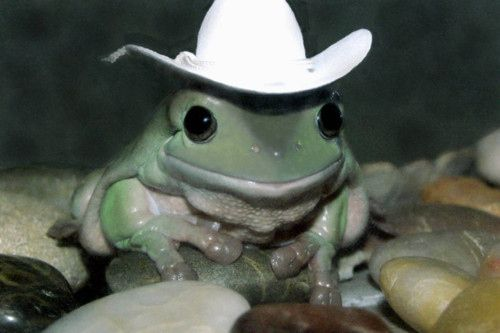
\includegraphics[width=\linewidth]{frog.jpg}
		\caption{\textit{This pond ain't big enough for the both of us.}}
		\label{fig:frog}
	\end{figure}

	\blindtext
	
	\section{RELATED WORK}
	
	\blindtext
	
	\begin{table}[h!]
	\centering
		\begin{tabular}{ |c|c|c| } 
		\hline
		American bullfrog & True toad & Tree frog \\ 
		Common frog & Barking tree frog & Pond frog \\ 
		Oak toad & Tomato frog & Pickerel frog \\ 
		\hline
		\end{tabular}
		\caption{Types of frogs.}	
	\end{table}

	\blindtext
	
	\section{METHOD}
	
	\blindtext
	\begin{table}[h!]
		\centering
		\begin{tabular}{ |c|c|c| } 
			\hline
			0 & 0 & 0 \\ 
			0 & 1 & 0\\ 
			0 & 0 & 1 \\ 
			\hline
		\end{tabular}
		\caption{These are binary numbers. The first row is 0. The second row is 2. The third row is 1. None of this really matters, but I am testing the formatting of a super long table name.}	
	\end{table}
	
	\blindtext
	
	\section{RESULTS, EVALUATION AND APPLICATIONS}
	
	\blindtext
	
	\section{CONCLUSION}
	
	\blindtext
\end{document}